%\section{One Feature Extraction Package to Rule Them All}
\section{The Largest Possible Survey of Features}
The NeuronUnit core, the Electrophysiology Feature Extraction Library \citep{EFEL}) EFEL, the Allen SDK, and the tests derived from \citep{druckmann2008evaluating} all contain independently written algorithms for computing features from simulated membrane potentials.
In some cases, the same feature (e.g. action potential threshold) is computed in many different ways across these feature extraction libraries.
All compute the threshold by first taking the first difference of the membrane potential, but they differ in subsequent steps, for example what value the first difference must reach to be considered at or beyond threshold.
This is inconvenient, but one can simply select one (or more) of the alternatives and apply it consistently.
More troubling are the cases where these algorithms differ in the stimulus used to generate the feature.
For example, the suprathreshold tests of \citep{druckmann2008evaluating} are based on a multiple of rheobase (e.g. $1.5\times$ or $3\times$), whereas those used by The Allen Insitute are based on additive increments from rheobase (e.g. +20 pA or +40 pA).
This means that cannot simply be applied to the same membrane potential trace, as those who collected the experimental data are likely to have chosen either multiples or additive increments of rheobase, but not both, depending on which lab they happen to work for.

As discussed in the Methods, I wrote code to restructure the Allen Cell Types and Blue Brain Project data sets, sorting traces into (approximate) multiples of rheobase, and the interpolating to select the sweep (in one data set) that is most appropriate for computing the feature defined in an otherwise-incompatible feature library.
In this way I was able to generate the same set of features from distinct datasets, even those that had use different stimuli.
%To make these conflicting lab protocols interoperable I impute 1.5 $\times$ and 3 $\times$ rheobase where it was not provided by finding the stimulus sweep pair that is the closest approximation. In this way I find the nearest traces to those predicted values in the Allen and BBP collections of sweeps.
One can conceive of more mathematically savvy types of imputation, and these could be the basis for future work.
If a more robust form of imputation was achieve, it could act as a Rosetta stone to link all the above feature extraction libraries together, allowing nearly any \emph{in vitro} dataset that is being collected data to be used to produce a canonical and universal set of features for model optimization.
%that is what I mean when I write imposing a new organisation on the sweep data.

% It may be possible to generate predicted features from one stimulus convention based on observed features from the other, allowing imputation of a full set of features across all algorithms, but this is beyond the scope of my thesis work. ISNT THIS WHAT I DID IN SOMEWAYS? IF I COULDN"T COMPARE ACROSS LAB PROTOCALS THEN THE ANALYSIS I DID WAS POINTLESS WAS IT NOT?

\section{Cross-Validation for Feature Selection: One Feature Set to Rule Them All}
The features identified during multivariate analysis utlilized the entire collection of models, data, and stimuli.
By contrast, a machine learning approach would have held out some of these for cross-validation, checking to see whether the features identified on a training set were in fact that features that best cluster, discriminate, or simply explain variance in the a held-out set of models and data.
For example, future work could identify a canonical set of stimuli and features fitness criteria, criteria that can train models to best satisfy multiple experimental protocols, rather than just one particular experiment.
These features would be shuffled (using stratification according to the stimuli that generated them) the objectives into ``train" and ``test" sets.
Cross-Validation may provide a strategy for dealing with conflicted features, such as the input resistance test.
If a trained model failed to score remotely well on such a test, this might identify that the model was overfit or simply that the test was unsatisfiable (given a model fit to the other tests).
This would allow for quick identification of which test combinations cannot work in practice, while also producing more generalizable models.

\section{Which is the Best Model Class for Producing Optimized Reduced Models?}
In previous spike-time prediction competitions \citep{incf_multi}, multi-time-scale variants of the AdEx model performed best.
It also had an admirable performance here, however the Izhikevich model was the overall winner.

Considering only features of at or below threshold spiking, the features that where used to get results below come from the tables 

By consulting tables: (\ref{tab:main_chi2},\ref{tab:HH_chi2}), and aggregating scores using python pandas, and averaging across $\chi^{2}$ statistics (which reflected 12 tests) for all neuron types, the Izhikevich model had the lowest mean $\chi^{2}$ (AdExp=$28.55$; Izhikevich=$1.39$), and the highest average $p-value$.
However, the Izhikevich model did not have the lowest $\chi^{2}$ for every cell type (see the Appendix for details).
%.when regarding each data set as a novel contest, the Adaptive Exponential lost to the Izhikevich model on two or more data sets see appendix \ref{appendix}.
%Adexp $28.55$ versus 
%Izhikevich $1.39$


The AdEx model suffered from its performance on the Olfactory Bulb Mitral Cell and the Cerebellum Purkinje cell (two of the largest cells types that were optimized). 
However, if you remove these two cells, and then judge the optimized models for the remaining cell types, the AdEx model is the winner by $\chi^{2}$ (AdExp=$0.51$; Izhikevich=$0.99$).

When consulting some of the traces for fitted models, it seemed as if either 1. AdExp and Izhikevich models lack the flexibility to model diverse cortical neuron activity, or 2. NeuroElectro data was difficult to fit.

% 
% In summary, the AdEx model is well-suited to cortical neuron types, but the Izhikevich model may have the flexibility to model the entire brain.

%The GLIF model was worse than both of the other model classes, and was limited in the same way as the AdEx model.
If you consider only Allen Cell Types data (all cortical neurons). On either of the following two sets of features:
\\

\begin{tabular}{|c|}
\toprule
Feature names \\
\midrule
RheobaseTest          \\
TimeConstantTest      \\
RestingPotentialTest  \\
InputResistanceTest   \\
\bottomrule
\end{tabular}
or:
\begin{tabular}{|c|}
\toprule
Feature names \\
\midrule
RheobaseTest \\
FITest      \\
\bottomrule
\end{tabular}
\\
\\
the GLIF model has $\chi^{2}=1.0$, however, if you consider other neurons (and tests)the mean $\chi^{2}$ value jumps to $364.2$.
The GLIF model were able to recapitulate FIslope exactly, however this caused conflicts with ability to fit time constant and rheobase, which was its downfall.
Even when the GLIF model was able to optimize cells to be within a biologically plausible range, simulation was slow and the quality of fits was not astounding.
It is unclear why anyone would choose to use this model outside of a very narrow range of applications.

Why did the Izhikevich model perform best?
I hypothesized that this was related to its broader coverage of dynamical regimes (as shown in \citep{izhikevich2003simple}).
To test this, I asked how many of these dozens of regimes were ``occupied" by the optimization solutions obtained here.
Specific optimization results (Section \ref{sec:appendix}).
I developed the izhikevich model, such that regime type was an explicit integer model parameter. Numbers 3-7 encoded regime types 1-7, where regimes 1,2,3 follow identical governing equations and so do not require unique numeric identifiers.
show that all but one of these regimes were occupied except for one associated with the activity of a dorsal LGN thalamocortical cell.
The ones associated with a barrel cortex low-threshold spiking (LTS) interneuron and a Layer 5 visual cortex fast-spiking (FS) interneuron were occupied the most often. 
%Regimes $1-3$ in this case representing the "regular-spiking" regime. A little surprisingly the regimes $1-3$ were only used in one fit Allen specimen $id-623960880$.


\section{Parameter Boundaries}
The error surface explored by the optimizer cannot extend infinitely far in all directions.
It must be initialized with boundaries that contain plausible parameter values.
If these boundaries are too narrow, they may exclude the optimal set of parameter values.
However, if they are too wide, then parameter sets that produce models well outside the range of biological plausibility will be produced.
Such implausible models undermine the assumptions of the features being calculated, and result in discontinuous or otherwise uninformative error surfaces where the optimizer wastes time exploring and may struggle to escape.
An example of parameter boundaries from the literature is shown in Figure \ref{fig:best_at_edge}.

\begin{figure}
    \centering
    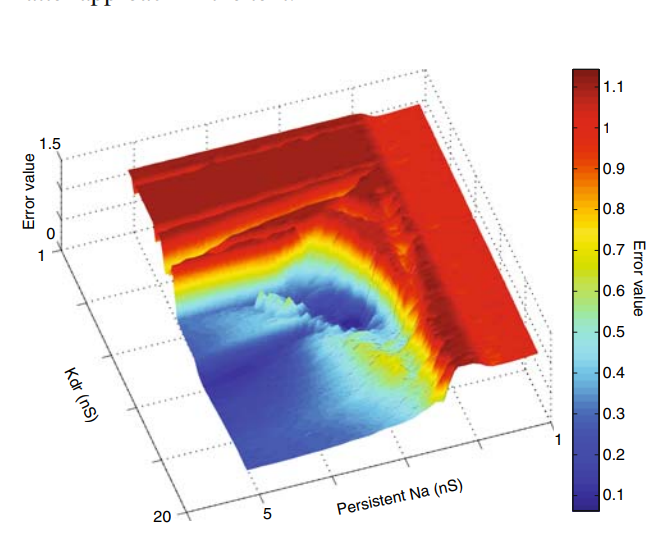
\includegraphics[scale=0.65]{figures/cliff.png}
    \caption[A plot of a cliff ledge framing a 2D error surface]{\textbf{Parameter boundaries can frame the search space}.
This error surface plot (from \cite{van2007neurofitter,van2008automated})
shows how the model/data agreement varies as two conductances from a biophysically-realistic conductance-based model are varied.
The large error values for $Na<2$ and $Kdr<2$ suggest that the decision not to search below the value 1 for either of these parameter was reasonable.
Similar grid searches could help to justify the parameter boundaries for optimization problems, provided that they can be conducted at low computational cost relative to optimization itself.}
    \label{fig:best_at_edge}
\end{figure}

For example, some parameter sets may cause a divergence in either the simulated membrane potential or in the features extracted from it.
This will be encoded as either ``not a number" (NaN) or $\inf$.
A single (NaN) or $\inf$ can infect the entire multiobjective function (i.e. any sum with $\inf$ will be $\inf$).
Because the optimizer can only succeed when it can distinguish better parameter sets from worse parameter sets, any chromosomes that get stuck in regions of parameter space with (NaN) or $\inf$ may not escape, even through mutation or crossover.
The error surface is locally ``flat" in a sense, and thus uninformative.
In order for the optimizer to survive the existence of such regions, the population size must be sufficiently large that a large number of chromosomes will avoid being initialized there.

In the opposite case, consider what might happen if the parameter boundaries are too narrow.
Figure \ref{fig:best_at_edge} shows another case from the literature, and in this case the global minimum error is positioned in a deep and narrow well.
It would be easy to have chosen parameter boundaries that miss this well entirely, resulting in a failure to obtain the optimal parameter set. 

\begin{figure}
    \centering
    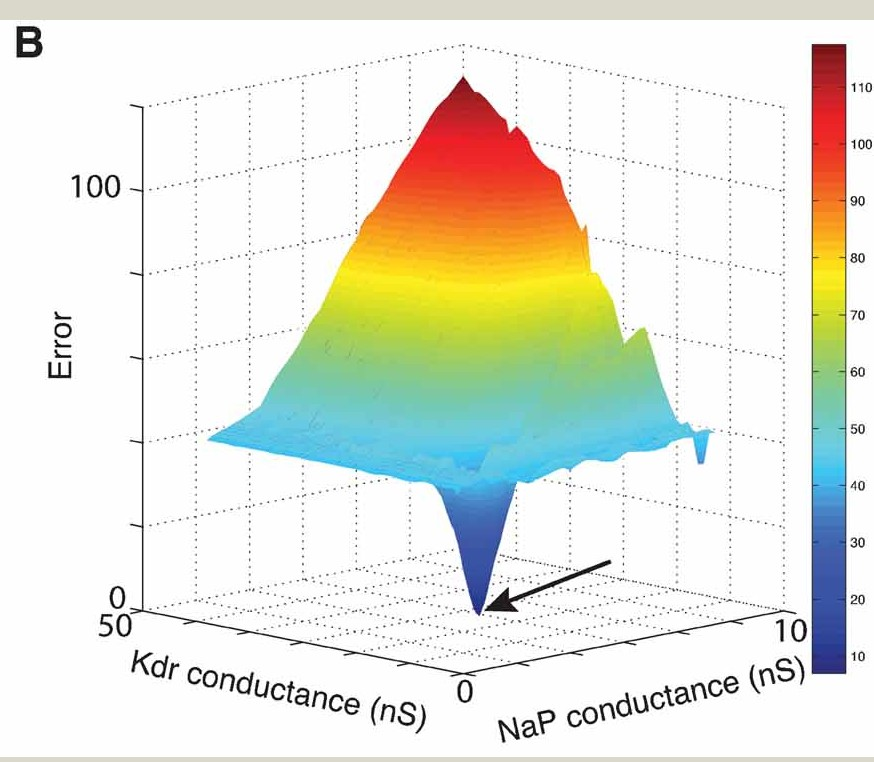
\includegraphics[scale=0.65]{figures/fninf-01-001-g009.jpg}
    \caption[A Challenging Location for the Optimal Value]{\textbf{A Challenging Location for the Optimal Value}.
    Again from \cite{van2008automated} I show an example of well-chosen parameter boundaries.
    These boundaries enclose the (narrow, deep) global minimum.
    Notably, choosing to explore only one quadrant of this space, where the error is roughly invariant to the parameter values, would have led to missing this global minimum entirely.}
    \label{fig:best_at_edge}
\end{figure}

A possible solution the problems above is to employ algorithms that peek beyond parameter boundaries and reports back on model stability.
This would be done only sparingly (otherwise it is equivalent to simply expanding the boundaries).
%In this manner one can do obtain the maximum parameter boundaries in an supervised computer algorithm, however, model equations used here, do exhibit some higher order sensitivity by changing a second intermediate parameter. Very quickly this approach to finding the maximum scope of a parameter may begin to look like exhaustive search.

%Another programmatic approach is to use a wide variety of models and tests, and to accept that for some model-test combinations, for some regions of parameter space, genetic algorithms are at worst randomly stumbling upon satisfactory solutions, and at best efficiently learning the optima solutions.


%The genetic algorithm
%As discussed, model-solution instability can occur when the optimizer samples model parameters that are outside of the models intended scope, or when a model returns a nan value inside its intended scope. It is tempting to think of 

%Usually these flat cliffs that neatly encase the error hyper volume like in the figure below \ref{fig:cliff} (and as described above).

% Not helpful for audiance to understand.
%unfortunately however, because each model has a large number of parameters typically $>10$, any particular model instance, only one of these parameters need be evaluating an unstable model when exceeding a margin, the rest of the parameters may be in the middle of their range, and so such a ledge may mostly be experienced as a hyper dimensional "tower", this tower could actually be experienced in the middle of parameter space in 10 out of 11 parameters, while still being on at the edge for only the 11th parameter. The unfortunate consequence of such towers is to lesion in the middle of parameter space inhibits the migration of chromosomes between regions. 

%From one perspective, the genetic algorithm is robust, and any middle region discontinuities are usually only a temporary hindrance that slows down learning without stopping it completely. From another perspective there are is only a small number of samples that occur inside the GA framework, and it would be better if the occurrence of lesions in the middle of the error surface were reduced to maximize the informativeness of every precious sample. 

%The major strategy for circumvent unnecessary ridges and towers is to pick and chose error functions sparingly and to assess results in a piecemeal basis. Utilizing a "sparing" inclusion policy will have to occur despite the large conflicting incentive to employ as many objective functions as possible.

% Picking the right objective functions will likely involve favoring a-posteri evidence over a-priori arguments about which errors "should" work best. 

%the majority of samples in the middle of the error space.

%To supplement figures from the literature, here I include some figures from problems encountered in this work.

%Although we are considering single points, and not surfaces, very often if a point is unstable, its neighbours are also unstable, in this way points of instability tend to be a constituents of larger regions of surface that add up to towers, cliffs and ledges such as those in seen here {fig:cliff}.

%One or more cliffs or towers situated in the middle of the error surface, poses problems for efficient optimization, where genes learn the general shape of an error surface. %Such cliffs and ledges will mislead the optimizer and they will act exactly like the ripples discussed briefly before in this work.

%Type \textbf{2}: While some towers can be circumvented by choosing slimmer parameter margins, other ledges and ripples of these ledges are implied by the types of model and test combinations. Rather than being avoidable, they are a feature of the complex problem that the optimizer is tasked with solving.

%Forinstance, in bursting regimes of the Izhikevich model, where models deliberately produce close to unstable limit cycles. When surpassing the threshold to cause spiking, the slightest increment of current  will illicit not a single spike but a burst of ten.

%Rheobase values will be undetermined, because the a  current injection value to that causes only one spike does not exist. The models rheobase value will be assigned to 100, and a tower will punctuate, the error surface possibly in the middle of the Izhikevich parameter hypervolume. The experience of sampling this tower, will visible in evaluation of the  algorithms learning performance. It will likely appear as a one or several unexpected peaks late in the genetic algorithms learning. Also this tower may act to lesion error surface, and to inhibit the movement of chromosomes across the solution space.

%This means that even under the most tractible conditions when evaluating the performance of genetic algorithm learning, the rapidity of genetic convergence will vary depending on which constraints are chosen, and the regime that the neuronal model is currently sampling from (the models parameters). There will be regions of genetic learning when models will encode high local pockets of error, or "towers" in the middle of the hyper-volume, and if these towers are significantly wide or densely populated, the genetic algorithms learning will be visibly diminished to a random sampling algorithm. What is more, these discontinuties under some circumstances may act to lesion error surfaces and inhibit migration of models from side to side. Movement over cliffs of course will still ultimately occur due to stochastic pressure in gene mutation.

